\documentclass[a4paper,12px]{article}
\usepackage{graphicx}
\usepackage[english]{babel}
\usepackage{fancyhdr}
\usepackage{lastpage}
\usepackage{xifthen}
\usepackage[linesnumberedhidden, titlenotnumbered]{algorithm2e}
\usepackage{lipsum}
\usepackage{hyperref}
\usepackage{array}
\usepackage{tabularx}
\usepackage{caption}
\usepackage{amsfonts}
\usepackage{amssymb}
\usepackage{amsmath}
\usepackage{placeins}
\usepackage{enumitem}

\usepackage{minted}
\usepackage{listings}
\usepackage{dsfont}
\usepackage{units}

\pagestyle{fancy}
\lhead{
\includegraphics[width=7cm]{logoUvA}}
\rhead{\footnotesize \textsc {Report\\ \opdracht}}
\lfoot
{%
    \footnotesize \studentA
    \ifthenelse{\isundefined{\studentB}}{}{\\ \studentB}
    \ifthenelse{\isundefined{\studentC}}{}{\\ \studentC}
    \ifthenelse{\isundefined{\studentD}}{}{\\ \studentD}
    \ifthenelse{\isundefined{\studentE}}{}{\\ \studentE}
}
\cfoot{}
\rfoot{\small \textsc {Page \thepage\ of \pageref{LastPage}}}
\renewcommand{\footrulewidth}{0.5pt}

\fancypagestyle{firststyle}
{%
    \fancyhf{}
    \renewcommand{\headrulewidth}{0pt}
    \chead{
\includegraphics[width=7cm]{logoUvA}}
    \rfoot{\small \textsc {Page \thepage\ of \pageref{LastPage}}}
}

\setlength{\topmargin}{-0.3in}
\setlength{\textheight}{630pt}
\setlength{\headsep}{40pt}
\setlength{\parindent}{0pt}

% =================================== DOC INFO ===================================

\newcommand{\opdracht}{Statistisch Redeneren}
\newcommand{\titel}{Lab 3}
\newcommand{\docent}{Rein van de Boomgaard}
\newcommand{\cursus}{Statistisch Redeneren}
\newcommand{\vakcode}{5062STRE6Y}
\newcommand{\datum}{\today}
\newcommand{\studentA}{Maico Timmerman}
\newcommand{\uvanetidA}{10542590}
\newcommand{\studentB}{Tim van Zalingen}
\newcommand{\uvanetidB}{10784012}
% \newcommand{\studentC}{Boudewijn Braams}
\newcommand{\uvanetidC}{10401040}
% \newcommand{\studentD}{Govert Verkes}
\newcommand{\uvanetidD}{10211748}
%\newcommand{\studentE}{Naam student 5}
\newcommand{\uvanetidE}{UvAnetID student 5}

% ===================================  ===================================

\begin{document}
\thispagestyle{firststyle}
\begin{center}
    \textsc{\Large \opdracht}\\[0.2cm]
    \rule{\linewidth}{0.5pt} \\[0.4cm]
    {\huge \bfseries \titel}
    \rule{\linewidth}{0.5pt} \\[0.2cm]
    {\large \datum  \\[0.4cm]}

    \begin{minipage}{0.4\textwidth}
        \begin{flushleft}

            \emph{Students:}\\
            {\studentA \\ {\small \uvanetidA \\[0.2cm]}}
            \ifthenelse{\isundefined{\studentB}}{}{\studentB \\ {\small \uvanetidB \\[0.2cm]}}
        \end{flushleft}
    \end{minipage}
    ~%
    \begin{minipage}{0.4\textwidth}
        \begin{flushright}
            \emph{Lecturer:} \\
            \docent \\[0.2cm]
            \emph{Course:} \\
            \cursus \\[0.2cm]
            % \emph{Student:}\\
            \ifthenelse{\isundefined{\studentC}}{}{\studentC \\ {\small \uvanetidC \\[0.2cm]}}
            \ifthenelse{\isundefined{\studentD}}{}{\studentD \\ {\small \uvanetidD \\[0.2cm]}}
            \ifthenelse{\isundefined{\studentE}}{}{\studentE \\ {\small \uvanetidE \\ [0.2cm]}}
        \end{flushright}
    \end{minipage}\\[1 cm]
\end{center}


% =================================== CONTENTS ===================================

\tableofcontents
\clearpage

% =================================== MAIN TEXT ===================================

\section{Lab Multivariate}
\subsection{19}
The expectation of \textbf{Z} is:
\begin{equation}
    \mu_z=\left( \begin{matrix}\mu_{x1}+\mu_{x2}\\\mu_{x1}-\mu_{x2}\end{matrix} \right)=
    \left(\begin{matrix}1-1\\1--1\end{matrix} \right)=
    \left(\begin{matrix}0\\2\end{matrix} \right)
\end{equation}
We can get \textbf{Z} by multiplying \textbf{X} in the following way:
\begin{equation}
    \label{eq:A_matrix}
    \text{\textbf{Z}}=\left(\begin{matrix}Z_1\\Z_2\end{matrix}\right)=
    \left(\begin{matrix}X_1+X_2\\X_1-X_2\end{matrix}\right)=
    \left(\begin{matrix}1&1\\1&-1\end{matrix}\right)\left(\begin{matrix}X_1\\X_2\end{matrix}\right)
\end{equation}
We can use this matrix that multiplies \textbf{X} to get \textbf{Z}, to get the
 covariance matrix:
\begin{equation}
    \Sigma_Z=\left(\begin{matrix}1&1\\1&-1\end{matrix}\right)
    \left(\begin{matrix}1&0\\0&4\end{matrix}\right)
    \left(\begin{matrix}1&1\\1&-1\end{matrix}\right)^T=
    \left(\begin{matrix}5&-3\\-3&5\end{matrix}\right)
\end{equation}
The covariance of $Z_1$ and $Z_2$ is not zero, so they are not independent.
\subsection{20}
First we calculate the covariance matrix for \textbf{Z}. We use the same matrix
 that multiplies \textbf{X} to get \textbf{Z} in equation \ref{eq:A_matrix}.
\begin{equation}
    \begin{aligned}
    \Sigma_Z&=\left(\begin{matrix}1&1\\1&-1\end{matrix}\right)
    \left(\begin{matrix}1&0\\0&c\end{matrix}\right)
    \left(\begin{matrix}1&1\\1&-1\end{matrix}\right)^T\\
    &=\left(\begin{matrix}1&1\\1&-1\end{matrix}\right)
    \left(\begin{matrix}1&1\\c&-c\end{matrix}\right)\\
    &=\left(\begin{matrix}1+c&1-c\\1-c&1+c\end{matrix}\right)
    \end{aligned}
\end{equation}
For the components of \textbf{Z} to be uncorrelated, the covariance of $Z_1$
 and $Z_2$ needs to be 0. This covariance is taken from $\Sigma_Z$.
\begin{equation}
    \begin{aligned}
    \text{cov}(Z_1, Z_2)=1-c&=0\\
    c&=1
    \end{aligned}
\end{equation}
\subsection{21}
The code for this exercise can be found in \textit{lab\_21.py}. Figure \ref{fig:21}
 shows the 12 scatter plots.
\begin{figure}
    \centering
    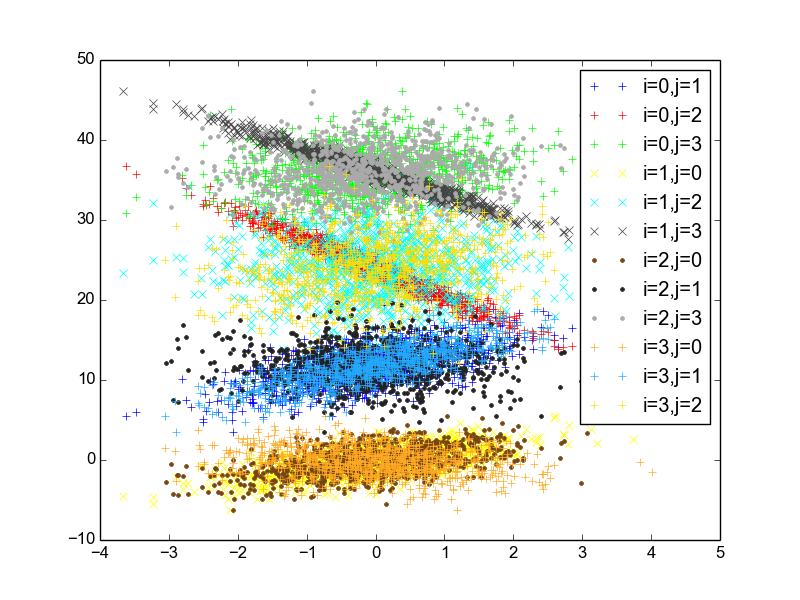
\includegraphics[width=1\textwidth]{fig21.png}
    \caption{12 scatter plots showing the non-diagonal elements from the data matrix}
    \label{fig:21}
\end{figure}
\FloatBarrier
\subsection{22}
Figure \ref{fig:22} shows us that for bigger N, the deviation in the covariance matrix
 and mean decrease. Which shows us that the accuracy of the estimators is dependent on N.
\begin{figure}
    \centering
    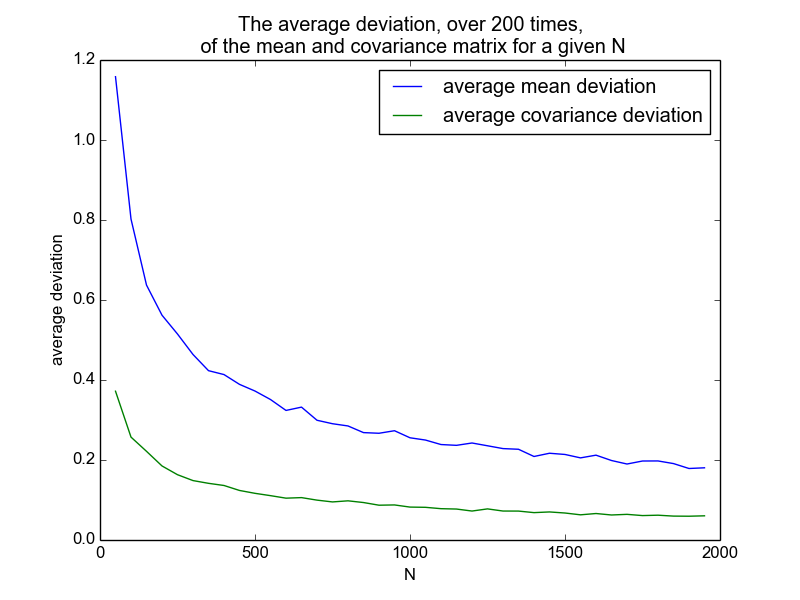
\includegraphics[width=1\textwidth]{fig22.png}
    \caption{}
    \label{fig:22}
\end{figure}
\FloatBarrier
When repeating the estimations for fixed N and collect the results in a data
 matrix, the covariance of this data matrix is the following:
\begin{equation}
\left(\begin{matrix}
  6.68374801 &   5.90243783 & -14.27310294 & -3.75627027\\
  5.90243783 &  11.73182492 & -20.63144665 &  1.7823714 \\
-14.27310294 & -20.63144665 &  49.69584792 & -8.45388543\\
 -3.75627027 &   1.7823714  &  -8.45388543 & 17.28203881\end{matrix}\right)
\end{equation}


\section{PCA}

\subsection{Incremental Calculation of the Covariance Matrix}

\begin{equation}
\begin{aligned}
S &= \frac{1}{n-1} \sum\limits_{i=1}^{n} (\vec x_i - \vec m)(\vec x_i - \vec m)^T\\
  &= \frac{1}{n-1} \sum\limits_{i=1}^{n} (\vec x_i - \vec m)(\vec x_i^T - \vec m^T)\\
  &= \frac{1}{n-1} \sum\limits^n_{i=1} \left(\vec x_i \vec x_i^T - \vec x_i \vec m^T -
                                             \vec m \vec x_i^T + \vec m \vec m ^T\right) \\
\end{aligned}
\end{equation}
To ease the proof, we leave $\frac{1}{n-1}$ out of the equation.
\begin{equation}
\begin{aligned}
  &= \sum\limits^n_{i=1} \left(\vec x_i \vec x_i^T - \vec x_i \vec m^T - \vec m \vec
    x_i^T + \vec m \vec m^T\right)\\
  &= \sum\limits^n_{i=1} \vec x_i \vec x_i^T - \sum\limits^n_{i=1} \vec x_i \vec m^T - \sum\limits^n_{i=1} \vec m \vec
    x_i^T + \sum\limits^n_{i=1} \vec m \vec m^T \\
  &= \sum\limits^n_{i=1} \vec x_i \vec x_i^T - \left(\sum\limits^n_{i=1} \vec x_i\right)
    \vec m^T - \vec m \left(\sum\limits^n_{i=1} \vec x_i\right)^T + n \vec m \vec m^T\\
\end{aligned}
\end{equation}
It is know that $\vec nm = \sum\limits_{i=1}^n \vec x_i$.
\begin{equation}
\begin{aligned}
    &= \sum\limits^n_{i=1} \vec x_i \vec x_i^T - n \vec m \vec m^T - n \vec m \vec
    m^T + n \vec m \vec m^T \\
\end{aligned}
\end{equation}
By adding $\frac{1}{n-1}$ back into the equation, we come to the following result.
\begin{equation}
\begin{aligned}
    S &= \frac{\left(\sum\limits^n_{i=1} \vec x_i \vec x_i^T \right) - n \vec m \vec m^T}{n-1} \\
\end{aligned}
\end{equation}

In the final equation, the matrix that is created by $\sum\limits_{i=1}^n \vec
x_i \vec x_i^T$ and the vector $\vec m$ can be calculated without loading the
entire data matrix in memory.

\subsection{EigenStructure}

Using the PCA method, it should be possible to describe local structures of a
photo with less data, while the reconstructed image still looks similar to the
original structure. Our implementation takes all possible samples of 25x25 to
calculate the covariance matrix. All these details can be described as vectors
of length 625, there are $232 \times 232 = 53824$ different details possible
for the images. This leads to a dataset of size 625 x 53824. The method from
the previous exercise is used, therefor not all the data needed to be loaded in
memory at the same time.


From the covariance matrix, the eigenvalue decomposition is calculated. These
eigenvalues are sorted in size, the see the most important dimension of
variance. As can be seen in \autoref{fig:eigenvalues}, the first eigenvalue's
value is triple on quadratic scale.

\begin{figure}[!h]
    \centering
    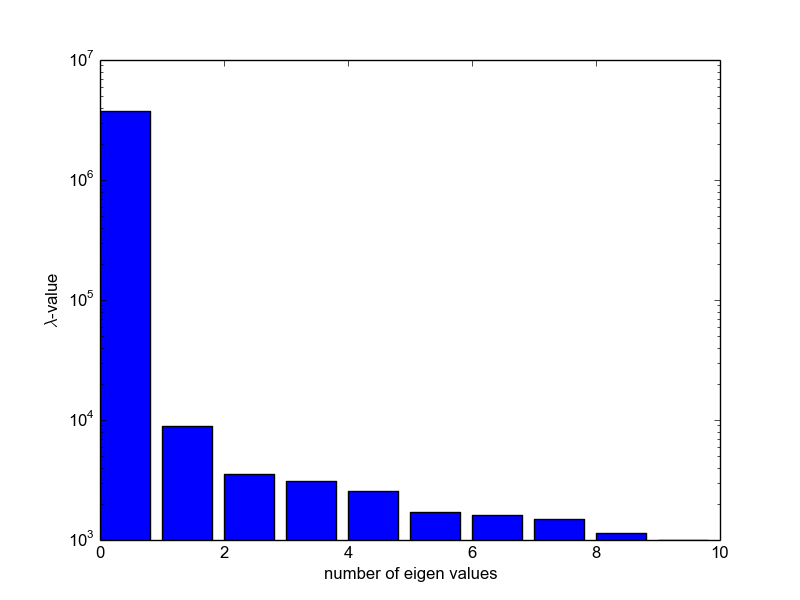
\includegraphics[width=\textwidth]{eigenvalues.png}
    \caption{Eigenvalues of the covariance matrix op \textit{trui.png}.}
    \label{fig:eigenvalues}
\end{figure}
\FloatBarrier

To reconstruct the image using the eigenvalues of the covariance matrix,
different number of original eigenvalues can be taken. To see the result of
reconstructed, we created the picture of reconstructed structures. As can be
seen in \autoref{fig:structures}, very small amount of eigenvalues gives a real
good view of the image.

\begin{figure}[!h]
    \centering
    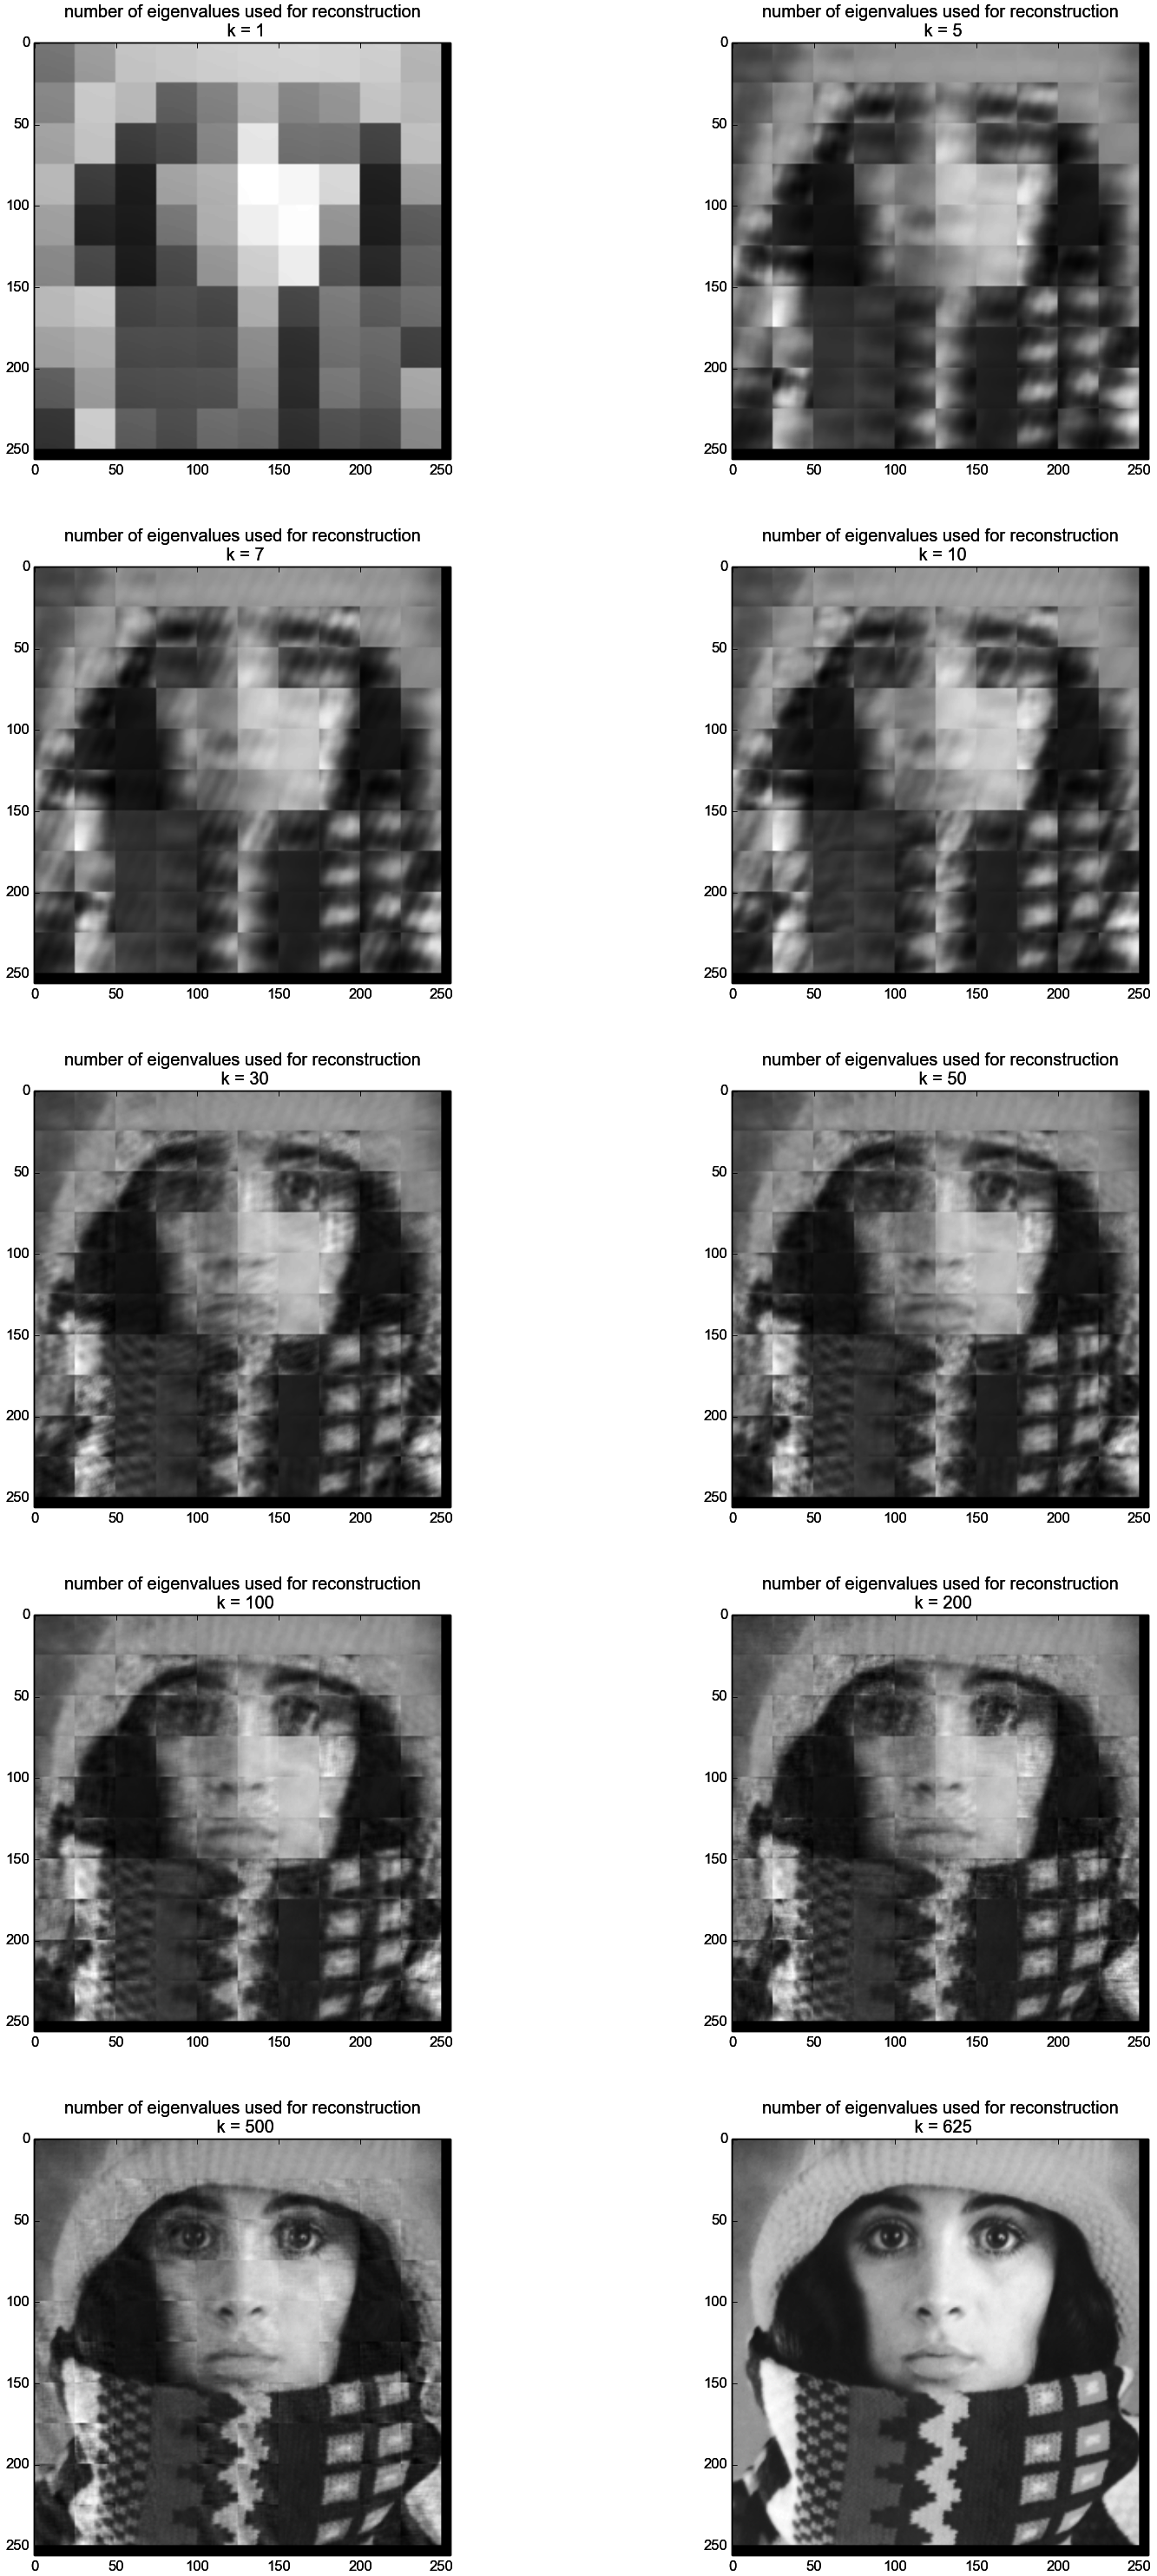
\includegraphics[width=0.8\textwidth]{montage.png}
    \caption{Reconstructed \textit{trui.png} from different number of eigenvalues.}
    \label{fig:structures}
\end{figure}
\FloatBarrier

% =================================== REFERENCES ===================================

%\clearpage
% \bibliographystyle{apalike}
% \bibliography{report}

\end{document}
